\documentclass[11pt]{article}
\usepackage[utf8]{inputenc}
\usepackage{polski}
\usepackage{graphicx}
\usepackage{array}
\usepackage{paralist}
\usepackage{verbatim}
\usepackage{subfig}
\usepackage{amsmath}
\usepackage{float}
\usepackage{amsthm}
\usepackage{amssymb}
\usepackage{pdfpages}
\usepackage{slashbox}
\usepackage{amsfonts}
\usepackage[margin=1in]{geometry}
\setlength\parindent{0pt}
\theoremstyle{definition}
\newtheorem{zadanie}{Zadanie}
\maxdeadcycles=1000
\extrafloats{1000}

\title{Podstawy układów logicznych - zadania z kolokwium}
\author{Igor Nowicki}
\begin{document}
\maketitle
\section{Caveat}

Zadania zostały ściągnięte ze zdjęć kolokwium z Podstaw Układów Logicznych na uczelni WIT. Rozwiazania zostały przygotowane na podstawie analizy slajdów Tadeusza Łuby oraz zdawkowych opisów w internecie. W związku z tym opisy mogą zawierać błędy. Używać na własną odpowiedzialność.

\section{Zadania}
\subsection{Zadanie 1}
\begin{zadanie}
Wyliczyć dopełnienie wyrażenia $ac+\overline a b$. Rozwiązanie podać w postaci sumy minimalnej liczby składników iloczynowych.
\end{zadanie}

\begin{proof}
Dopełnienie wyrażenia oznacza negację całości:

$$\overline{(ac+ \overline ab)}.$$

Negacja sumy jest równa iloczynowi negacji:

$$\overline{ac} \cdot \overline{\overline a b}.$$

Ponownie, negacja iloczynu jest równa sumie negacji:

$$(\overline a+\overline c)(a+\overline b).$$

Wymnażamy obydwa wyrażenia:

$$\overline aa+ \overline a\overline b + a\overline c + \overline b\overline c$$

Iloczyn wartości i jej negacji jest zawsze zerowy:

$$\overline a\overline b + a\overline c + \overline b\overline c$$

Mamy trzy argumenty, z których środkowy jest kombinacją dwóch skrajnych. Skorzystamy z tożsamości $\overline c + c = 1$ i zmienimy ostatni argument na:

$$
\overline a\overline b + a\overline c + (a+\overline a)\overline b\overline c
=
\overline a\overline b + a\overline c + a\overline b\overline c + \overline a\overline b\overline c
$$

Połączymy pierwszy wyraz z czwartym i drugi z trzecim:

$$\overline a\overline b+ \overline a\overline b\overline c + a\overline c + a\overline b\overline c = \overline a\overline b(1+\overline c) + a(1+\overline b)\overline c$$

Cokolwiek dodane do $1$ zwraca $1$, zatem $1+\overline b = 1$.

$$ \overline a\overline b(1+\overline c) + a(1+\overline b)\overline c =  \overline a\overline b + a\overline c$$


\end{proof}


\subsection{Zadanie 2}
\begin{zadanie}
Zminimalizować funkcję metodą Karnaugh'a.

$$y = \sum \big(3,4,10,15,(1,6,8,9,11,12,14)\big)$$
\end{zadanie}

\begin{proof}
Ponieważ mamy maksymalne pole równe 15, oznacza to że możemy funkcję zapisać za pomocą czterech zmiennych ($2^4 = 16$, wartości od 0 do 15). Nazwiemy je $a,b,c,d$.

Minimalizacja funkcji metodą Karnaugha polega na stworzeniu tabeli z kolumnami i wierszami numerowanymi kodem Graya:


\begin{table}[H]
\begin{tabular}{|c|c|c|c|c|}
\hline
\backslashbox{cd}{ab} &$00$ & $01$ & $11$ & $10$ \\
\hline 00&&&&\\
\hline 01&&&&\\
\hline 11&&&&\\
\hline 10&&&&\\
 \hline
\end{tabular}
\end{table}

Następnie ponumerujemy pola wewnątrz tabeli, używając wartości binarnych zbudowanych z oznaczeń binarnych kolumn i wierszy:


\begin{table}[H]
\begin{tabular}{|c|c|c|c|c|}
\hline
\backslashbox{cd}{ab} &$00$ & $01$ & $11$ & $10$ \\
\hline 00&\tiny{0}&\tiny{1}&\tiny{3}&\tiny{2}\\
\hline 01&\tiny{4}&\tiny{5}&\tiny{7}&\tiny{6}\\
\hline 11&\tiny{12}&\tiny{13}&\tiny{15}&\tiny{14}\\
\hline 10&\tiny{8}&\tiny{9}&\tiny{11}&\tiny{10}\\
 \hline
\end{tabular}
\end{table}

Następnie wypełniamy pola wartościami z równania funkcji. Ponieważ mamy symbol $\sum$, oznacza to mamy numery pól o wartości $1$. W wewnętrznym nawiasie mamy natomiast numery pól niezdefiniowanych, z wartościami $-$. Reszta pól przyjmuje wartość $0$.


\begin{table}[H]
\begin{tabular}{|c|c|c|c|c|}
\hline
\backslashbox{cd}{ab} &$00$ & $01$ & $11$ & $10$ \\
\hline 00&0&-&1&0\\
\hline 01&1&0&0&-\\
\hline 11&-&0&1&-\\
\hline 10&-&-&-&1\\
 \hline
\end{tabular}
\end{table}

Minimalizacja metodą Karnaugh'a polega teraz na stworzeniu jak największych prostokątnych zbiorów zawierajacych jedynki i kreski. Zbiory muszą mieć liczbę pól równą wielokrotnościom dwójki (1,2,4,8,16, etc.) i odpowiadają implikantom prostym funkcji logicznej.

\begin{figure}[H]
\centering
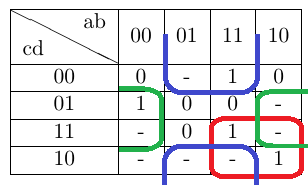
\includegraphics[width=0.5\linewidth]{tab_1.png}
\end{figure}


Mamy trzy prostokąty - czerwony, zielony, niebieski - z których dwa byłyby prostokątami gdyby spiąć pierwszą i czwartą kolumnę oraz pierwszy i czwarty wiersz razem. Dla czerwonego prostokąta element $a$ ma niezmienną wartość $1$ (element $b$ się zmienia), element $c$ ma również wartość $1$, zmienna $d$ się zmienia. Oznacza to że czerwony prostokąt odpowiada wyrażeniu $ac$.

Wykonując podobne operacje dla zielonego ''prostokąta'' widzimy, że element $b$ ma stałą wartość $0$ oraz element $d$ ma wartość 1. Odpowiada to wyrażeniu $\overline bd$.

Niebieski prostokąt będzie odpowiadał wyrażeniu $b\overline d$.

Łącząc te trzy wyrażenia w sumę, uzyskujemy rozwiązanie:

$$f = ac + \overline bd + b\overline d.$$
\end{proof}

\subsection{Zadanie 3}
\begin{zadanie}
Dany jest wektor $k_i$ ze zbioru $F$ oraz zbiór $R$. Znaleźć wszystkie implikanty proste dla $k_i$.

$$k_i = [1, 1, 0, 1, 1]$$

$$R = 
\begin{vmatrix}
1&0&0&1&0 \\
0&0&0&1&0 \\
-&1&0&0&0 \\
1&1&1&0&1 \\
0&0&1&0&1
\end{vmatrix}
$$
\end{zadanie}

\begin{proof}
Będziemy tu korzystali z części algorytmu ekspansji metody Espresso. Algorytm polega na podzieleniu tabeli funkcji logicznej na części odpowiadające $f=1$ (nazwaną dla zmyłki $F$) oraz $f=0$ (nazwaną $R$). Z części $F$ bierzemy kolejne wiersze $k_i$ i używamy ich do negowania tych kolumn macierzy $R$ które odpowiadają wartosciom $1$ z wiersza $k_i$. W ten sposób tworzymy macierz $B(k_i, R)$. Dla uproszczenia wszelkie $-$ zastąpimy pod koniec wartościami $0$:

$$B(k_i, R) = 
\begin{vmatrix}
0&1&0&0&1 \\
1&1&0&0&1 \\
0&0&0&1&1 \\
0&0&1&1&0 \\
1&1&1&1&0
\end{vmatrix}
$$

Zanegowałem tutaj kolumny 1,2,4 i 5, ponieważ w wektorze $k_i$ na tych polach miałem wartości 1.

Teraz bierzemy dla każdego wiersza z macierzy $B$ numery kolumn na których mamy wartość 1. Będą one odpowiadać wartościom $x_1$ do $x_5$ które zsumowane dadzą nam części iloczynu.


$$B(k_i, R) = 
\begin{vmatrix}
0&1&0&0&1 \\
1&1&0&0&1 \\
0&0&0&1&1 \\
0&0&1&1&0 \\
1&1&1&1&0
\end{vmatrix} \qquad \begin{matrix} x_2+x_5\\x_1+x_2+x_5\\x_4+x_5\\x_3+x_4\\x_1+x_2+x_3+x_4\end{matrix}
$$

Aby uprościć obliczenia, na samym początku skreślamy wiersze będące rozszerzeniem innego wiersza - w tym wypadku drugi wiersz jest pierwszym wierszem z dodanym elementem $x_1$, natomiast wiersz piąty jest tożsamy z wierszem czwartym (+ $x_1+x_2$). Pozostałe sumy z wierszy wymnażamy:

\begin{align*}
(x_2+x_5)(x_4+x_5)(x_3+x_4) &= (x_2x_4 + x_2x_5+x_4x_5 + x_5)(x_3+x_4),\\
 &= (x_2x_4 + x_5)(x_3+x_4),\\
 &= x_2x_3x_4 + x_2x_4 + x_3x_5 + x_4x_5,\\
 &= x_2x_4 + x_3x_5 + x_4x_5.
\end{align*}

Zatem implikanty proste to $x_2x_4$, $x_3x_5$ oraz $x_4x_5$.


\end{proof}

\subsection{Zadanie 4}

\begin{zadanie}
Dla funkcji podanej w tablicy obliczyć wszystkie minimalne zbiory argumentów z najmniejszą liczbą argumentów. Zmienne niezbędne tej funkcji to $x_5, x_{10}$.

\begin{table}[H]
\begin{tabular}{|c|c|c|c|c|c|c|c|c|c|c|c|c|}
\hline
 &$x_1$ & $x_2$ & $x_3$ & $x_4$ &$x_5$ &$x_6$ &$x_7$ &$x_8$ &$x_9$ &$x_{10}$  & y  \\
 \hline  1&1&1&1&0&0&0&1&1&1&0&0  \\
 \hline  2&1&0&0&0&1&0&1&0&0&0&0  \\
 \hline  3&1&0&1&1&1&1&1&0&1&0&1  \\
 \hline  4&1&0&0&0&0&0&1&0&0&0&1  \\
 \hline  5&0&1&0&0&0&1&0&1&1&1&1  \\
 \hline  6&1&1&0&0&0&0&0&1&1&0&1  \\
 \hline  7&1&0&0&0&1&0&1&0&0&1&1 \\
 \hline
\end{tabular}
\end{table}

\begin{proof}
Zadanie wymaga od nas użycia algorytmu redukcji argumentów. Szczęśliwie mamy podane zmienne niezbędne dla tej funkcji logicznej. Tworzymy wektory $P_5$, $P_{10}$ z kolumn $x_5$, $x_{10}$.

\begin{align*}
P_5 &= [0,1,1,0,0,0,1],\\
P_{10} &= [0,0,0,0,1,0,1].
\end{align*}

Dodatkowo tworzymy wektor $P_f$ na podstawie kolumny $y$, gdzie mamy rozdzielone pola $0$ oraz $1$:

$$P_f = (1,2)(3,4,5,6,7).$$

Tworzymy iloczyn $P_N = P_5\circ P_{10}$, rozdzielający na cztery zbiory numery kolumn w których wartości odpowiadają wartościom z kolum $00, 01, 10, 11$.

$$P_N = (1,4,6) | (2,3) | (5) | (7)$$

(pierwszy zbiór to kolumny gdzie wartości były równe $00$, drugi: $10$, trzeci: $01$, czwarty: $11$).

Rozdzielamy każdy ze zbiorów w $P_N$ według $P_F$ - na części należące do pierwszego i drugiego zbioru $P_f$:

$$P_N\circ P_f = (1)(4,6) \quad\big|\quad (2)(3) \quad\big|\quad (5)\quad \big|\quad (7)$$

Dla każdej pary zbiorów w jednym polu tworzymy kombinacje: $1|4$, $1|6$, $2|3$. Dla tych wartości bierzemy pary wierszy o tych numerach z początkowej tabeli i podajemy numery kolumn na których są różne wartości elementów:

\begin{align*}
1|4 &=x_2 + x_3+x_8+x_9\\
1|6 &=x_3+x_7\\
2|3 &=x_3+x_4+x_6+x_9
\end{align*}

Sumy te wymnażamy ze sobą:

\begin{align*}
(x_2 + x_3+x_8+x_9)(x_3+x_7)(x_3+x_4+x_6+x_9) = \\
(x_2x_3 + x_3 + x_3x_8+x_3x_9 + x_2x_7+x_3x_7+x_7x_8+x_7x_9)(x_3+x_4+x_6+x_9) = \\
(x_3 + x_2x_7+x_3x_7+x_7x_8+x_7x_9)(x_3+x_4+x_6+x_9) =\\
\end{align*}
\begin{align*}
x_3+x_3x_4+x_3x_6+x_3x_9 + x_2x_3x_7 +x_2x_4x_7+x_2x_4x_7+x_2x_6x_7+x_2x_7x_9 + \\
x_3x_7+x_3x_4x_7+x_3x_6x_7+x_3x_7x_9+x_3x_7x_8+x_4x_7x_8s+x_6x_7x_8+x_7x_8x_9+\\
x_3x_7x_9+x_4x_7x_9+x_6x_7x_9+x_7x_9
\end{align*}

Ten koszmarek szczęśliwie można skrócić, korzystając z tożsamości $a + ab = a(1+b) = a$ oraz $a+a = a$:

\begin{align*}
x_3+x_7x_9+x_2x_4x_7+x_2x_6x_7+x_4x_7x_8+x_6x_7x_8
\end{align*}

Bierzemy wyrażenia o najmniejszej liczbie argumentów-  w tym wypadku będzie to zmienna $x_3$. Mogliśmy do tego dojść również analizując wcześniejsze równania i zauważając że $x_3$ jest jedyną zmienną która pojawia się we wszystkich trzech wierszach. Ostateczny minimalny zbiór argumentów (po dodaniu zmiennych niezbędnych $x_5, x_{10}$ to $\{x_3, x_5, x_{10}\}$.


\end{proof}

\end{zadanie}
\end{document}